\documentclass[10pt]{article}

\usepackage[a4paper,left=20mm, right=20mm, top=20mm, bottom=20mm]{geometry}
\usepackage{pdfpages}
\usepackage{markdown}
\usepackage{multicol}
\usepackage{caption}
\usepackage[none]{hyphenat}

\title{2-way Concrete Speaker Documentation}
\author{Eero Talus}
\date{\today}

\begin{document}
\maketitle
\tableofcontents

\section{License}

\begin{sloppypar}
\noindent
\texttt{Copyright Eero Talus 2020.}\\

\noindent
\texttt{This documentation describes Open Hardware and is licensed under the
CERN OHL v. 1.2.}\\

\noindent
\texttt{You may redistribute and modify this documentation under the terms of
the CERN OHL v.1.2. (http://ohwr.org/cernohl). This documentation is distributed
WITHOUT ANY EXPRESS OR IMPLIED WARRANTY, INCLUDING OF MERCHANTABILITY,
SATISFACTORY QUALITY AND FITNESS FOR A PARTICULAR PURPOSE. Please see the
CERN OHL v.1.2 for applicable conditions.}
\end{sloppypar}

\section{Introduction}

\noindent This PDF contains documentation for my self designed vented two way
speakers. All the design files can be found from the GIT repository at
\url{https://github.com/eerotal/2-way-speaker}. Below is a 3D render of the
speakers.\\

\begin{figure}[htp]
	\centering
	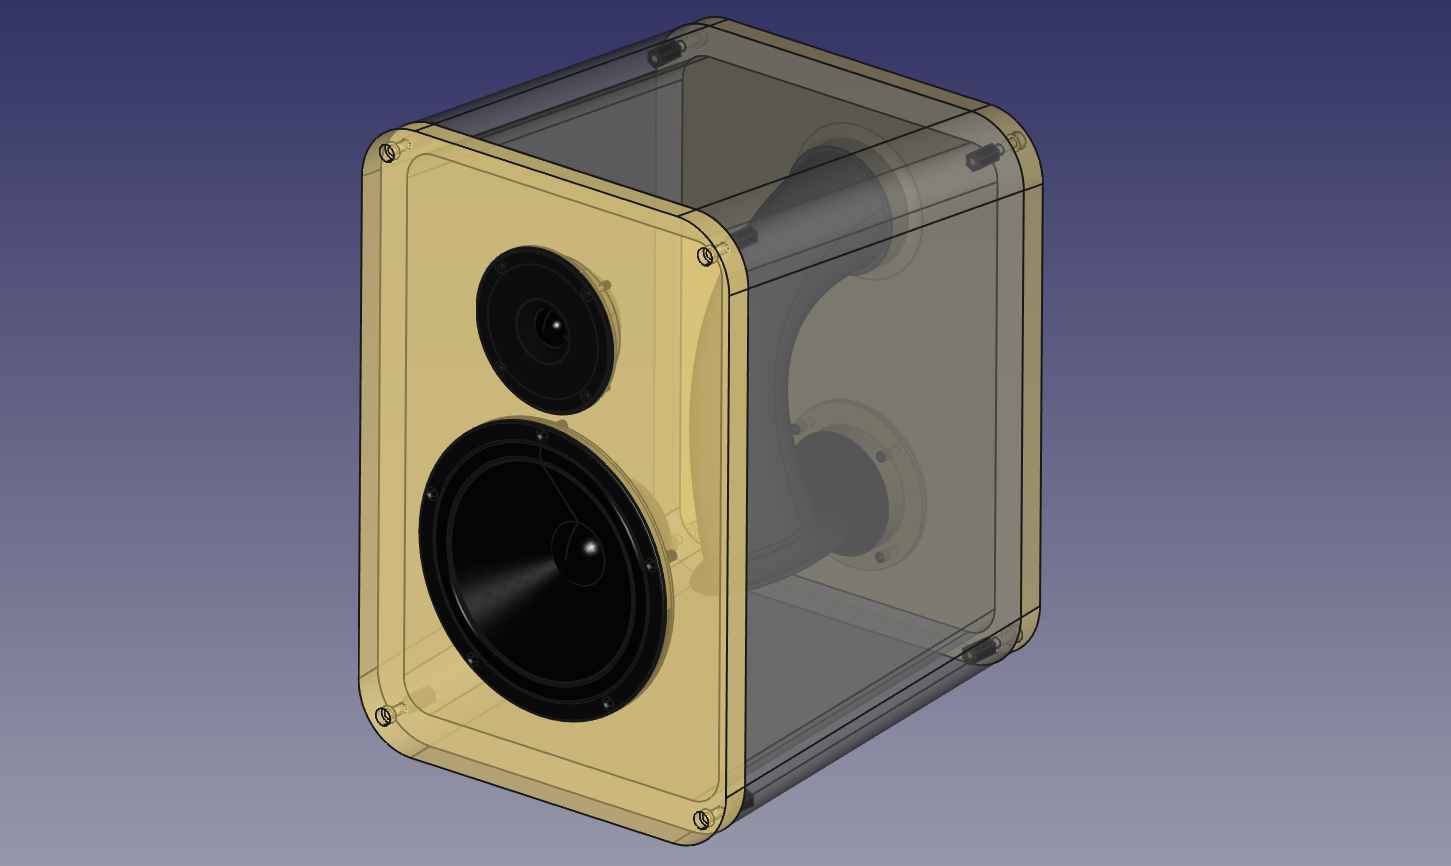
\includegraphics[width=0.9\textwidth]{../drawings/render.png}
	\caption{3D render of the speaker.}
\end{figure}

\begin{figure}[htp]
	\centering
	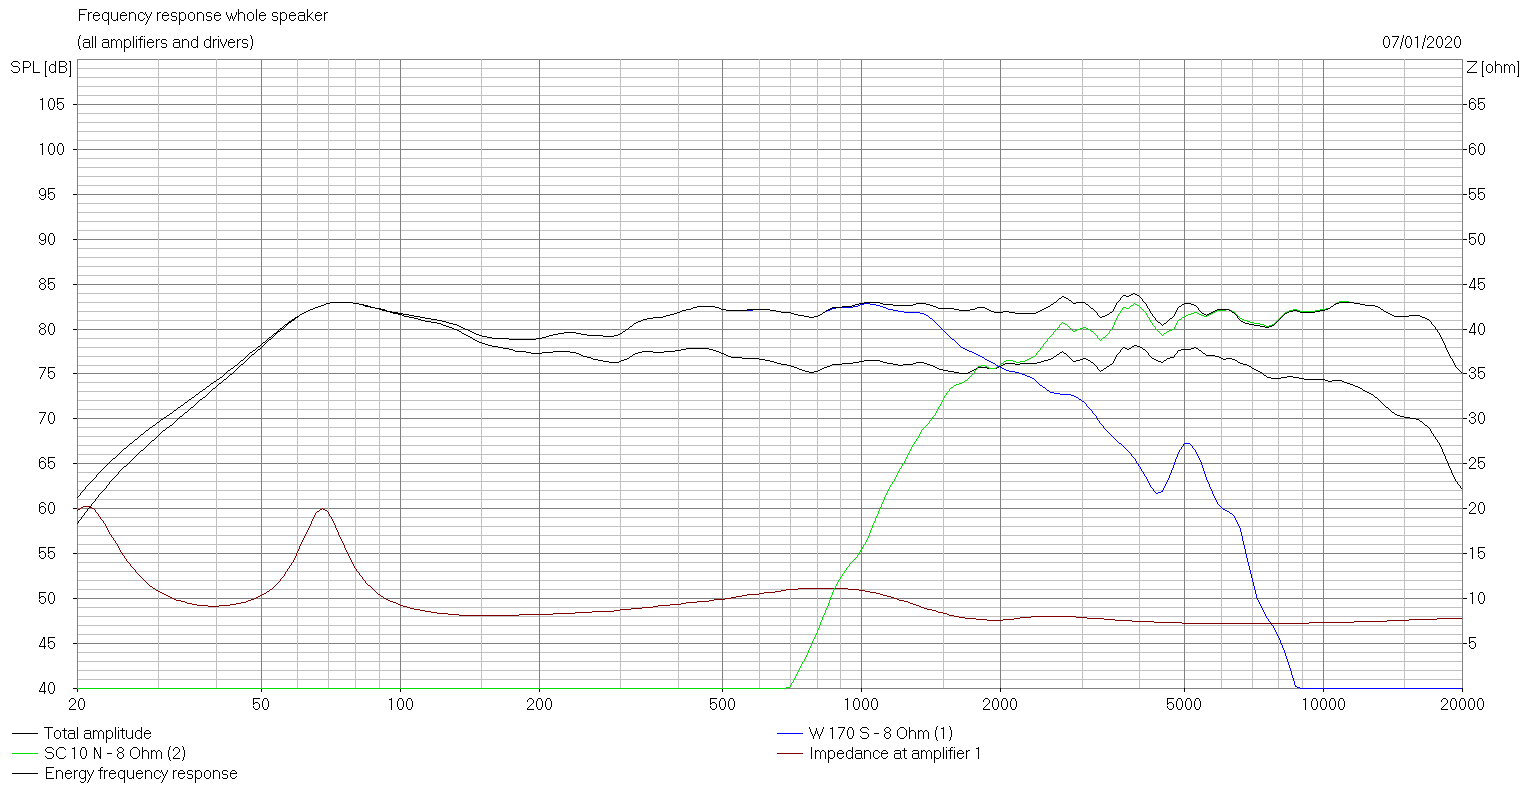
\includegraphics[width=0.9\textwidth]{../drawings/Frequency_Response.png}
	\caption{Speaker frequency response graph.}
\end{figure}

\pagebreak

\noindent The speaker specifications are:

\begin{itemize}
\item Cabinet volume (V): 20 l
\item Cabinet tuning frequenxy (Fb): 42.49 Hz
\item Woofer: Visaton W-170 S 8Ohm
\item Tweeter: Visaton SC-10 N
\end{itemize}

\noindent The speaker cabinet was designed to have a frequency response that's
as flat as possible over the entire bandwidth of the speaker. The cabinet
features a theoretically optimal reflex port designed based on various research
papers on the subject. The cabinet is constructed from concrete and wood to
increase its mass and to improve speaker performance.\\

\noindent The speaker uses a crossover circuit made using third order
Butterworth filters. Speaker impedance and sensitivity matching was also taken
into account while desiging the filter. All design and documentation files were
created using open file formats, tools and technologies.\\

\noindent You can run the shell script \texttt makedocs.sh to generate this
PDF file.

\section{Respository directory structure}

\begin{itemize}
\item 2-way-speaker
    \begin{itemize}
    \item crossover
        \begin{itemize}
        \item KiCad
            \begin{itemize}
            \item \textit{Crossover schematics and PCB design files.}
            \end{itemize}
        \item ngspice
            \begin{itemize}
            \item \textit{NgSpice crossover simulation files.}
            \end{itemize}
        \end{itemize}
    \item docs
        \begin{itemize}
        \item \textit{Documentation files.}
        \end{itemize}
    \item latex
        \begin{itemize}
        \item \textit{LaTeX files for concatenating all documentation files into one PDF.}
        \end{itemize}
    \item math
        \begin{itemize}
        \item \textit{WxMaxima design calculations.}
        \end{itemize}
    \item models
        \begin{itemize}
        \item \textit{FreeCAD 3D design files.}
        \end{itemize}
    \item simulation
        \begin{itemize}
        \item \textit{Visaton Boxsim simulation files.}
        \end{itemize}
    \end{itemize}
\end{itemize}

\section{Software and technologies}

Below is a list of the software and technologies used in this project.

\begin{itemize}
\item KiCad: Crossover electronics design.
\item ngspice: Crossover circuit simulation.
\item FreeCAD: 3D models and mechanical drawings.
\item Boxsim: Speaker simulation.
\item wxMaxima: Design calculations.
\item LaTeX: Documentation
\end{itemize}

\pagebreak
\null
\vfil
\centering\section{Mechanical drawings}
\vfil
\pagebreak
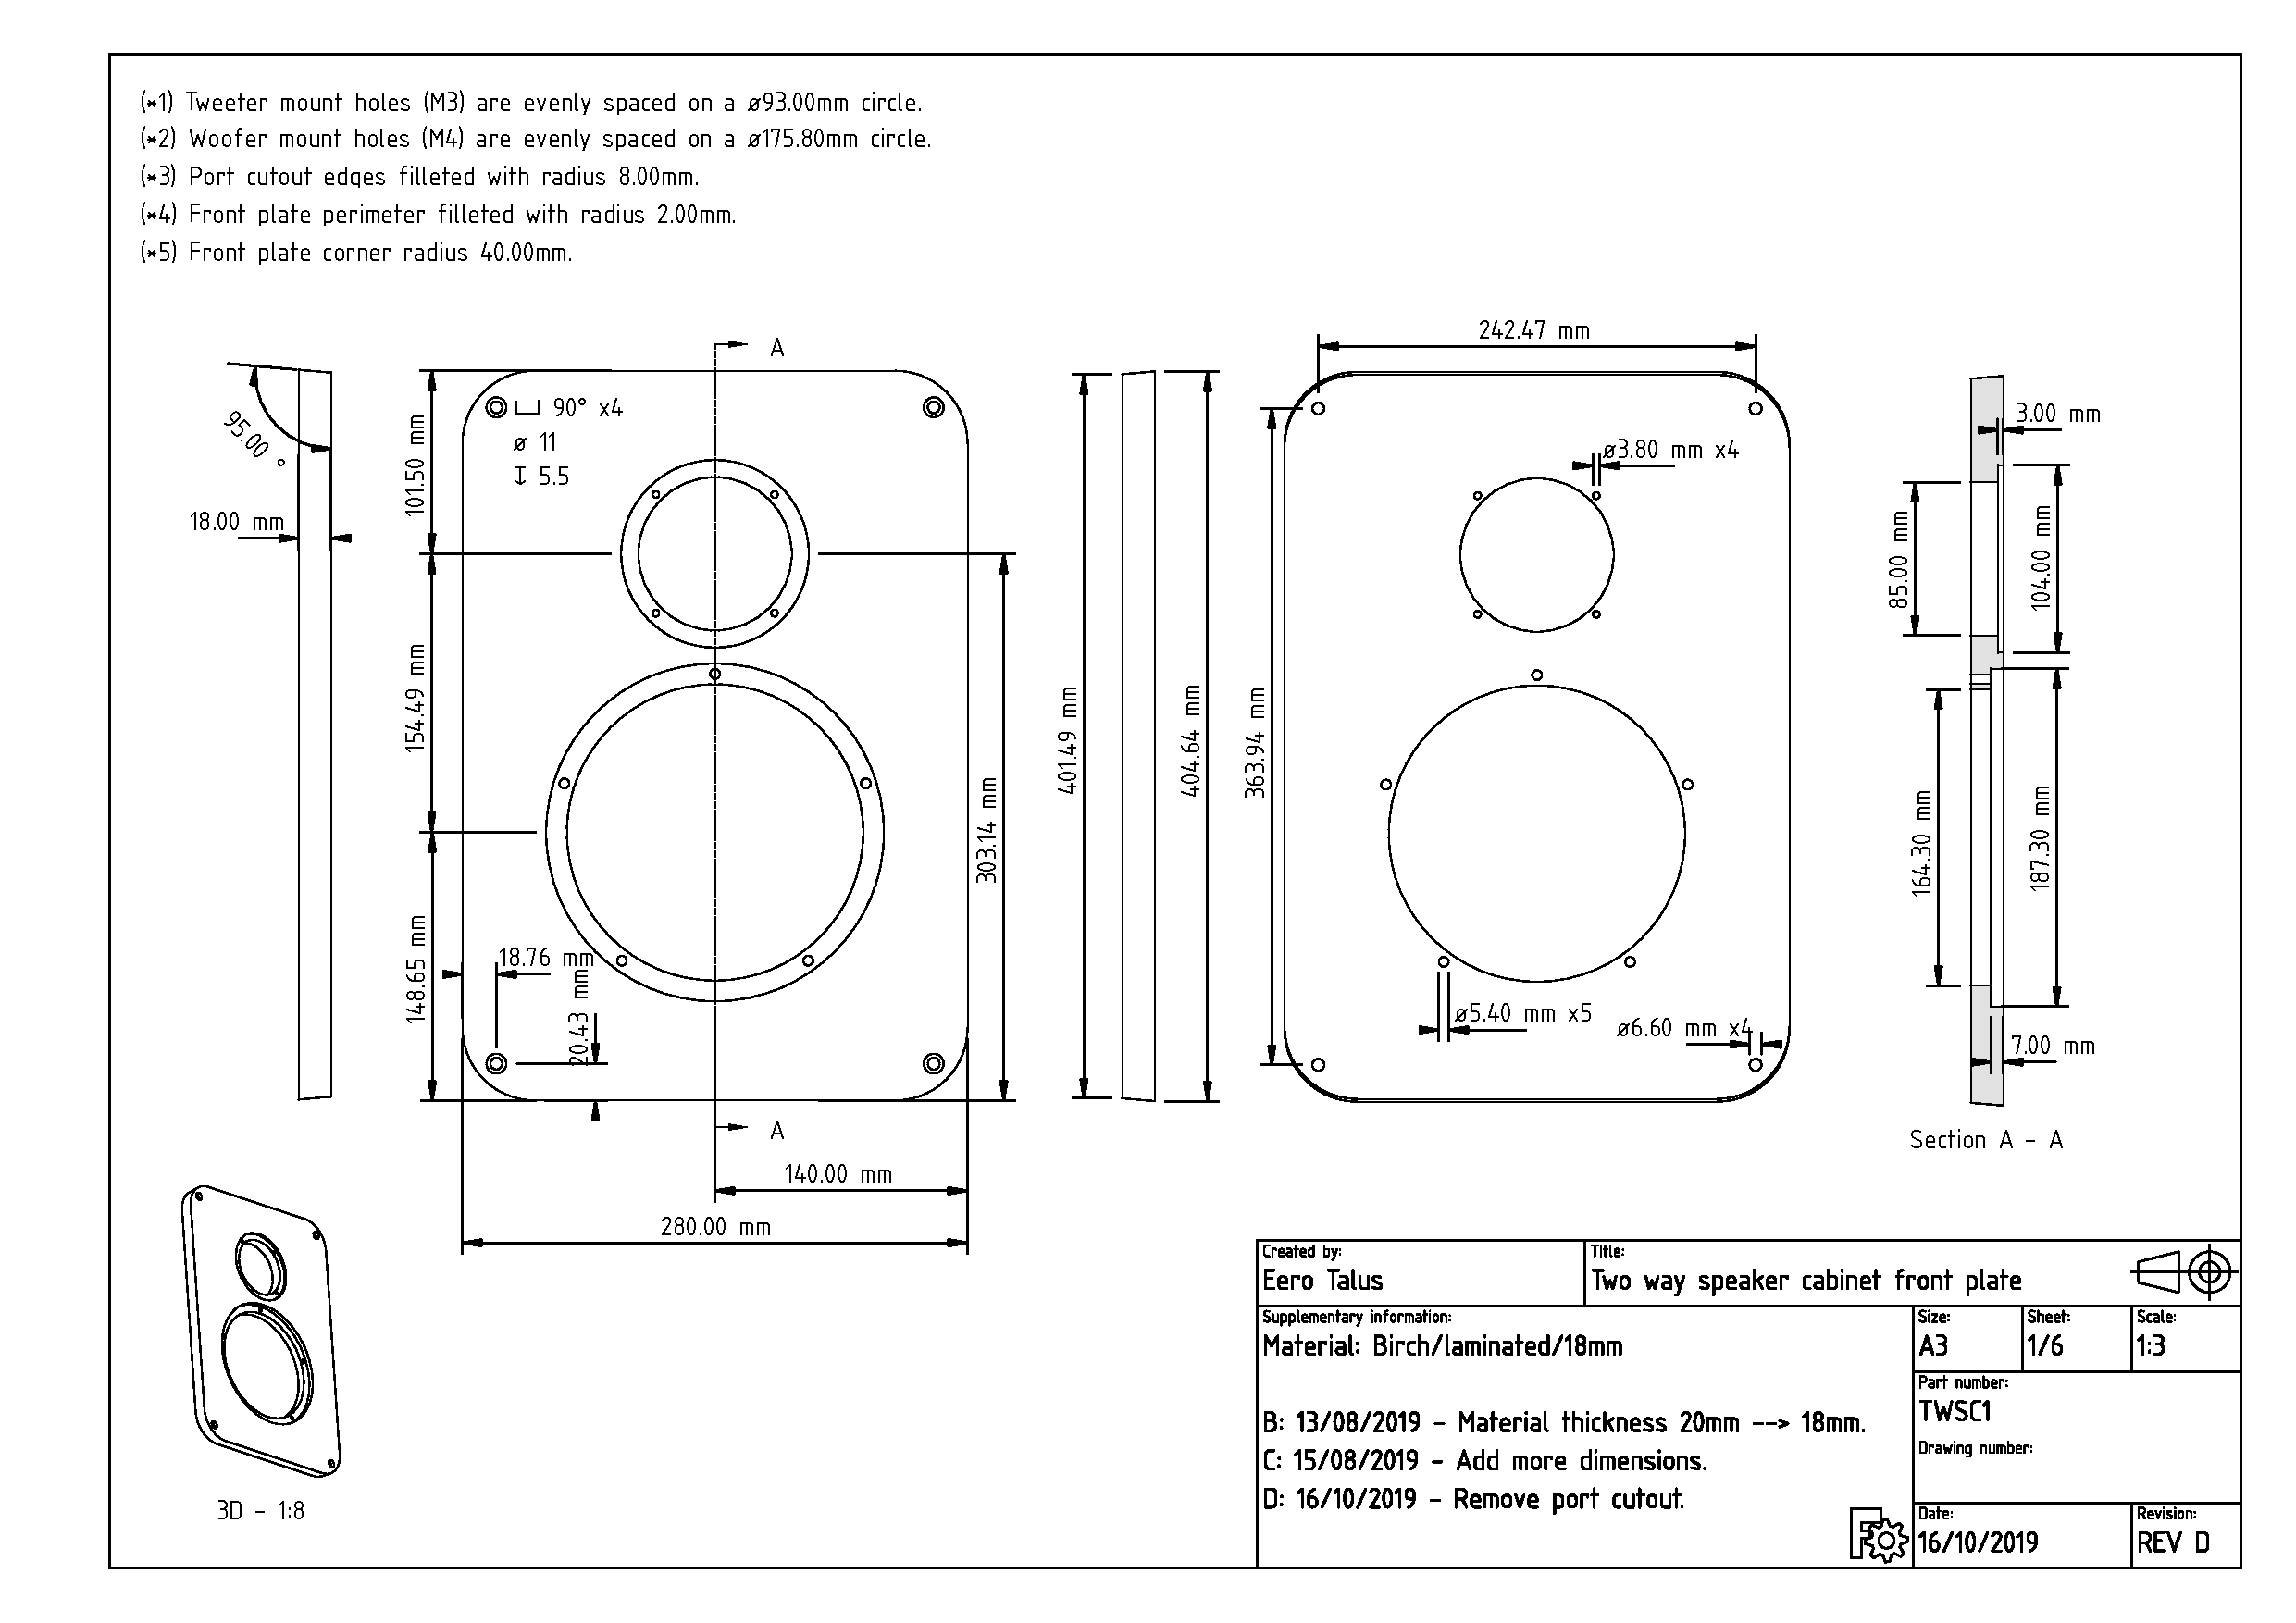
\includepdf[landscape=true]{../drawings/Front_Plate_Drawing.pdf}
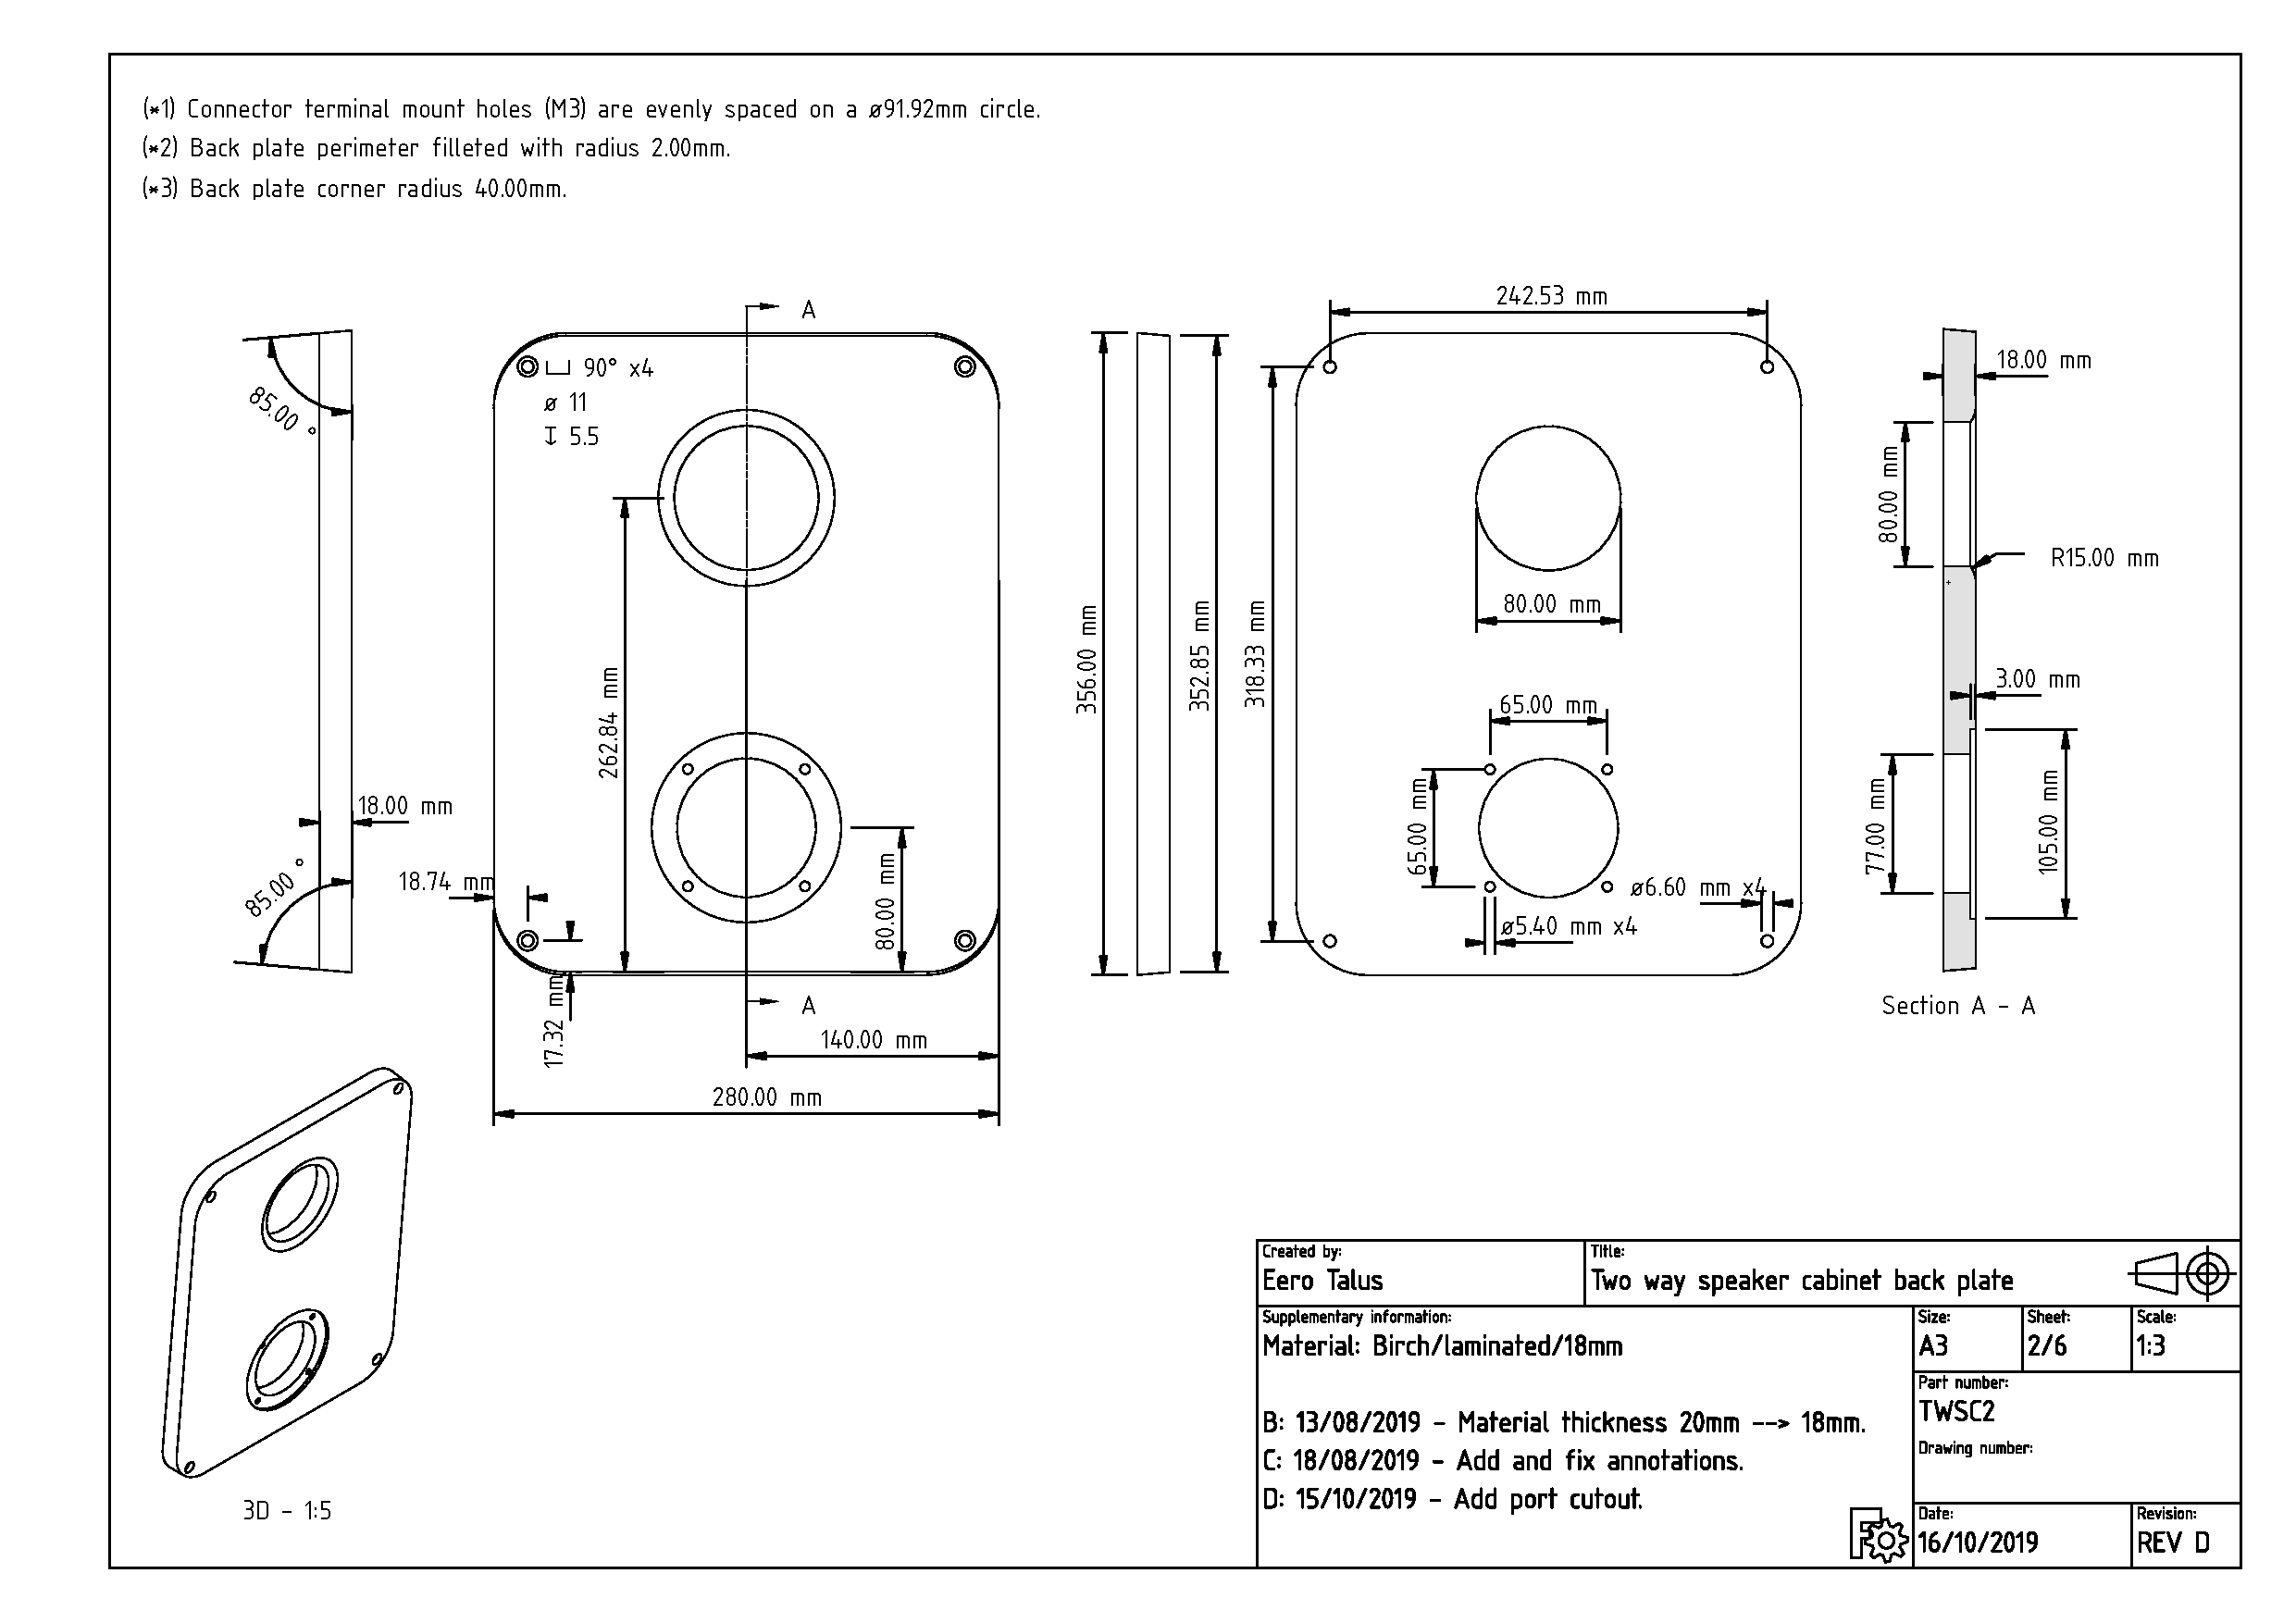
\includepdf[landscape=true]{../drawings/Back_Plate_Drawing.pdf}
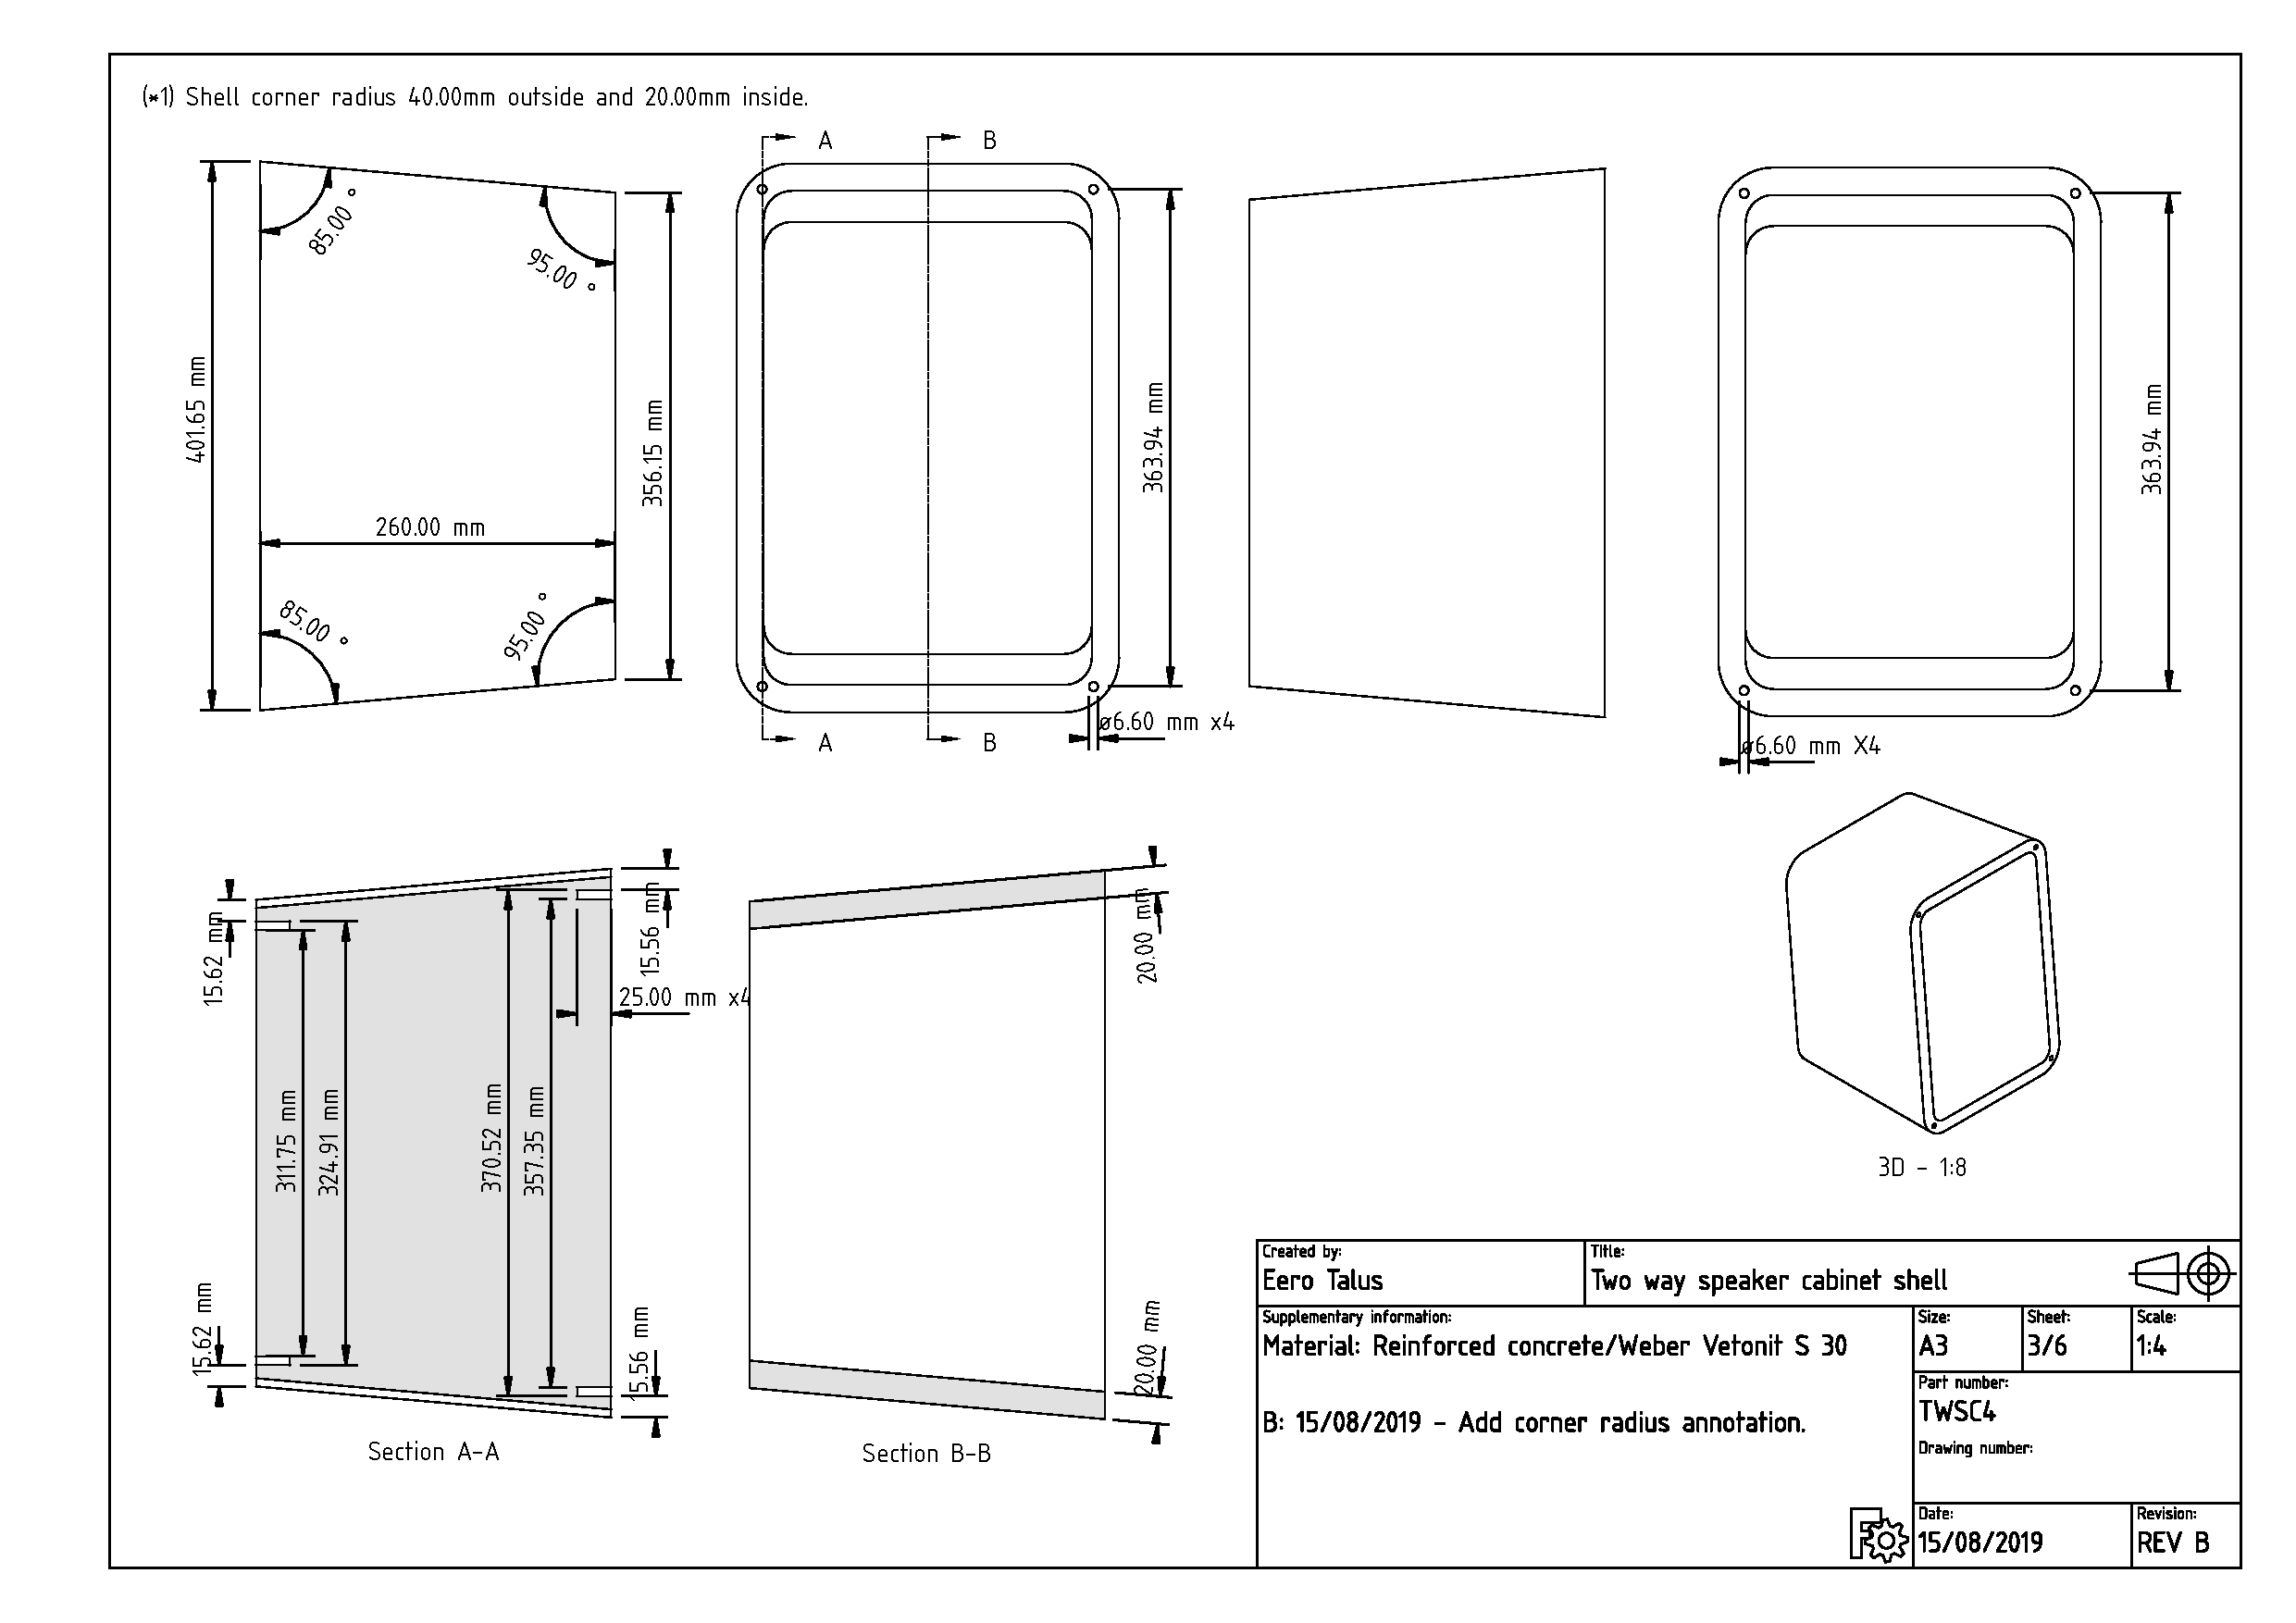
\includepdf[landscape=true]{../drawings/Shell_Drawing.pdf}
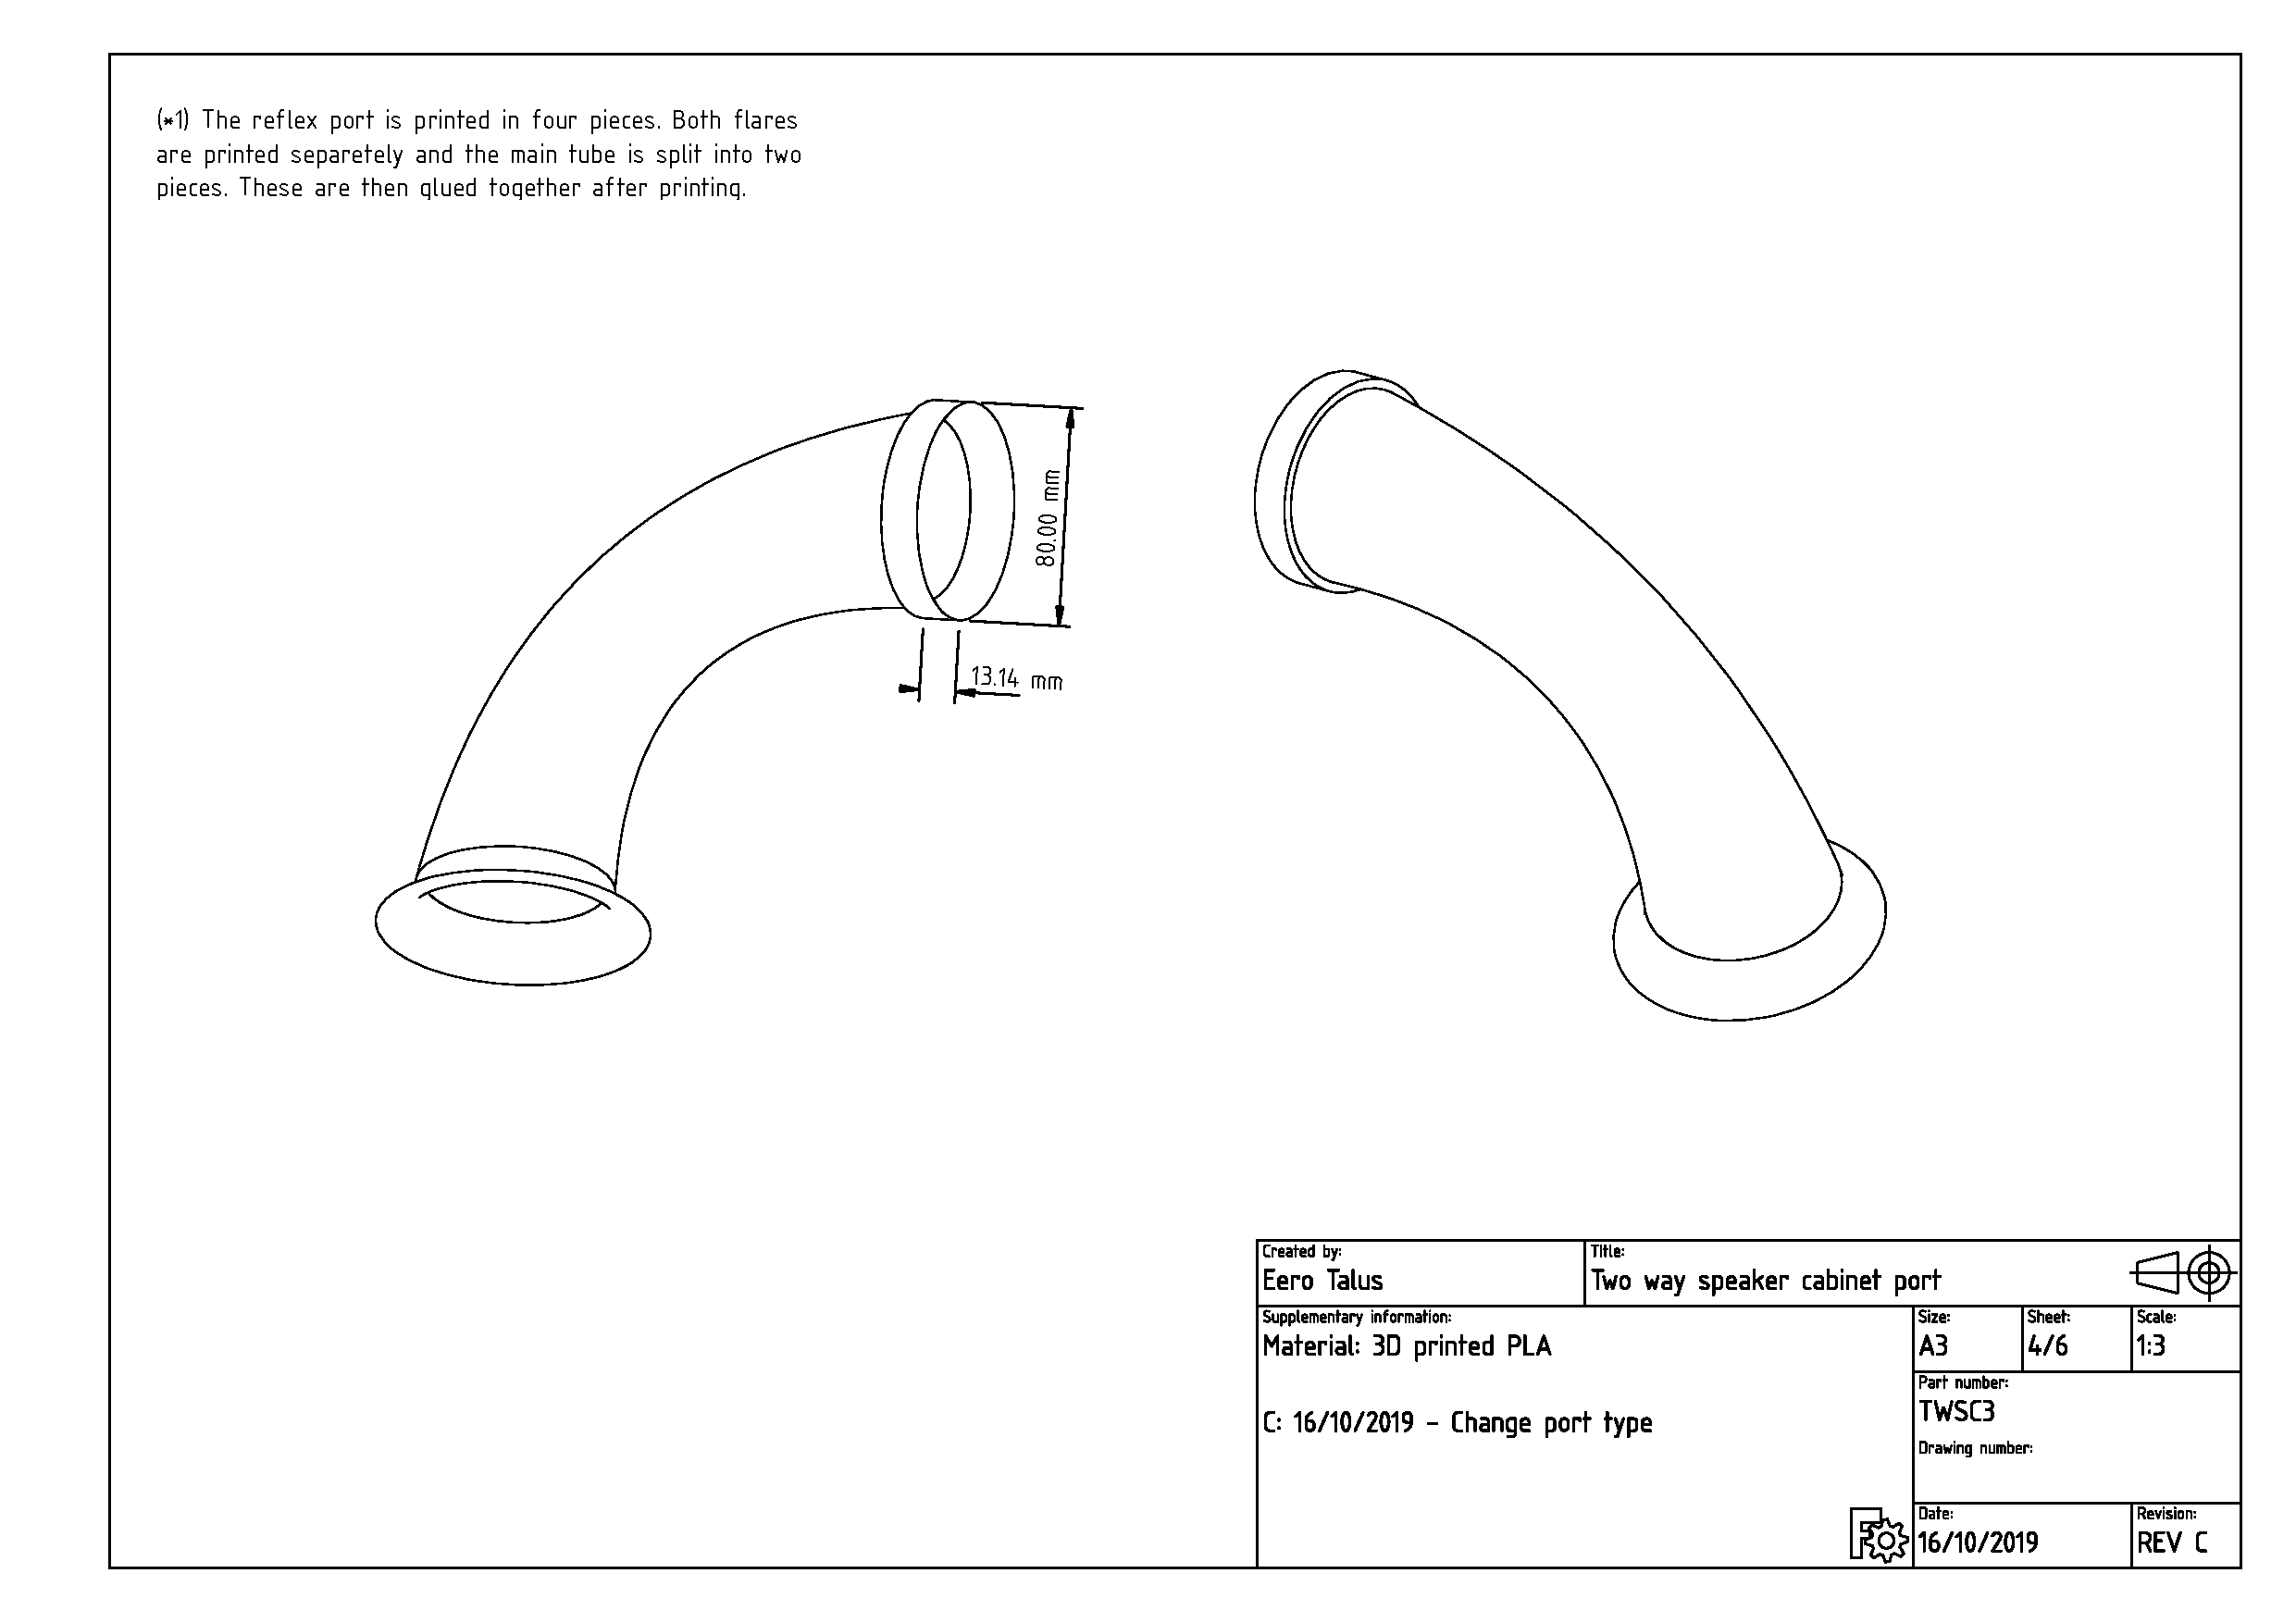
\includepdf[landscape=true]{../drawings/Port_Drawing.pdf}

\pagebreak
\null
\vfil
\centering\section{Crossover schematic and simulation graphs}
\vfil
\pagebreak
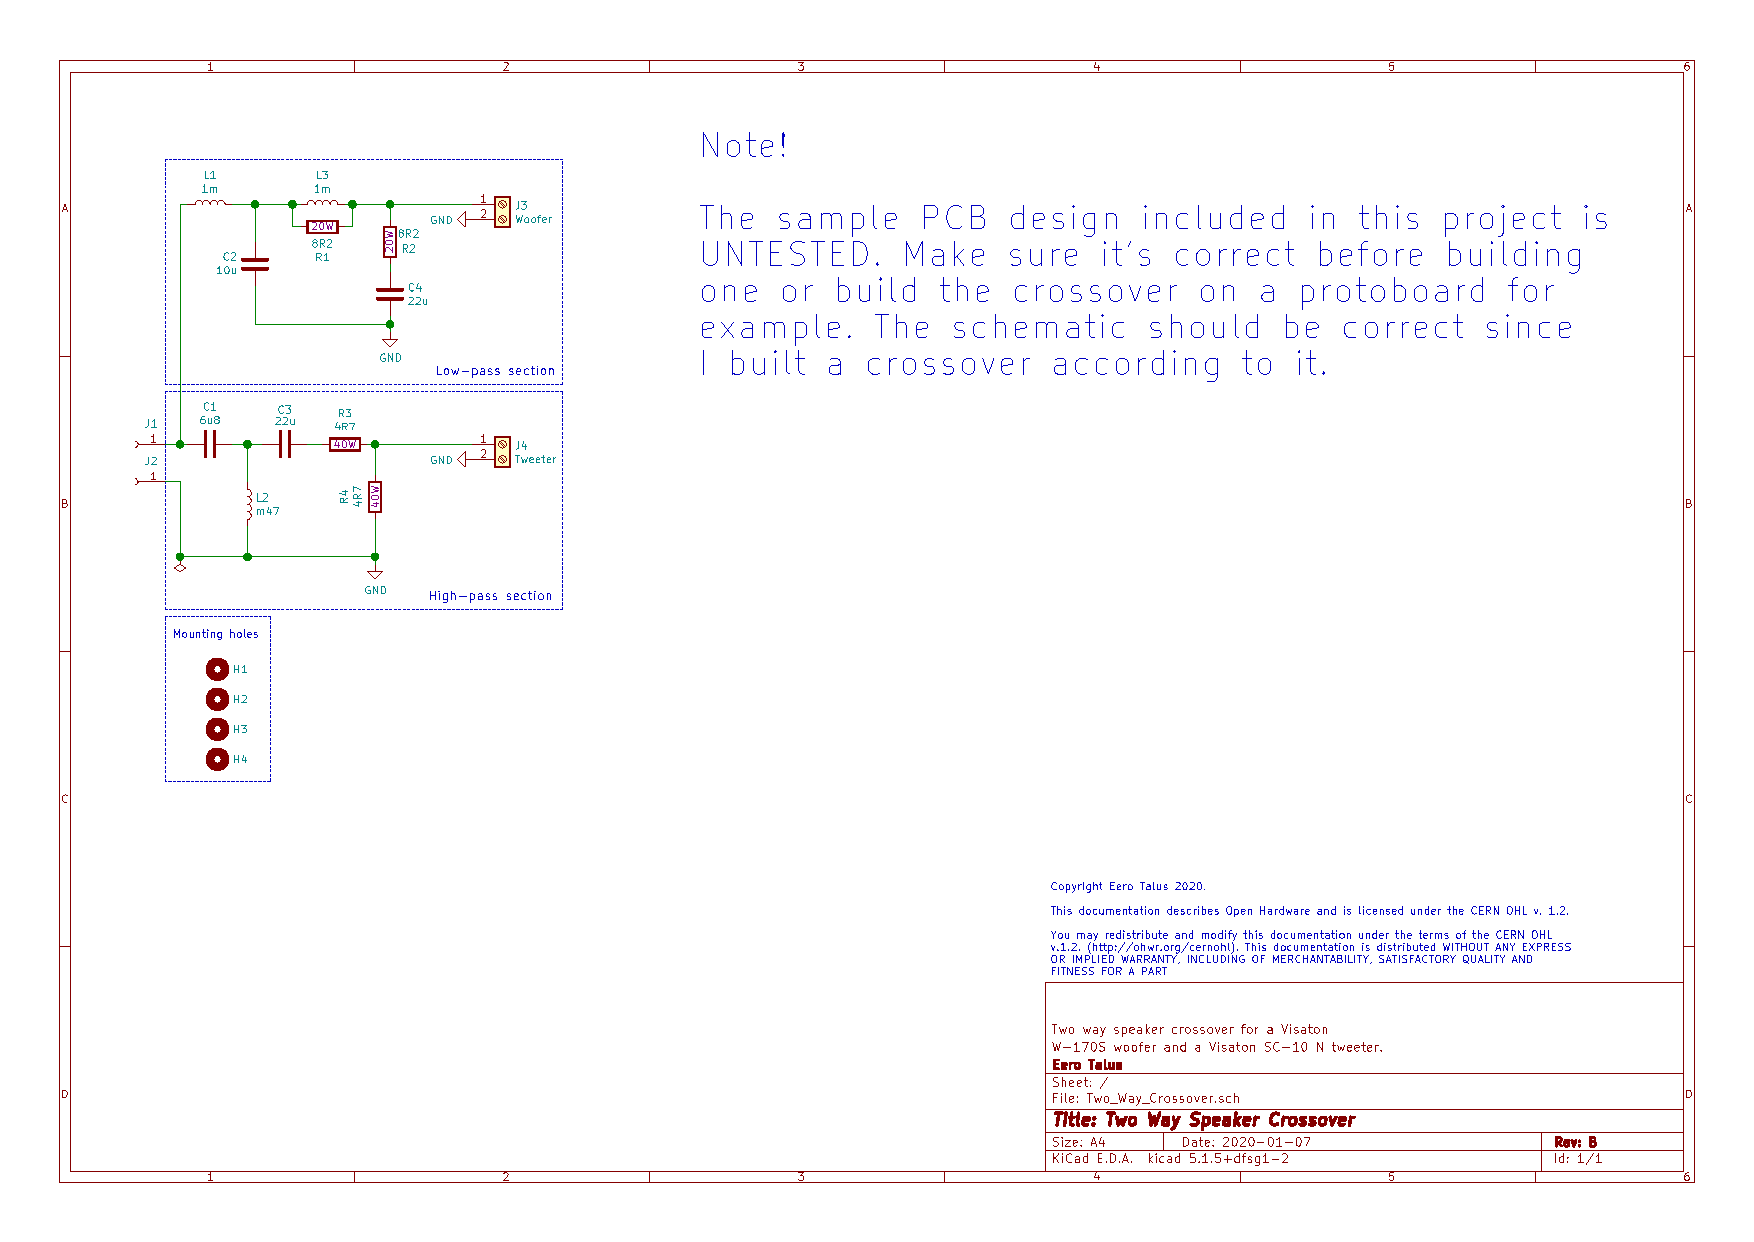
\includepdf[landscape=true]{../drawings/Crossover_Schematic.pdf}
\begin{multicols}{2}
	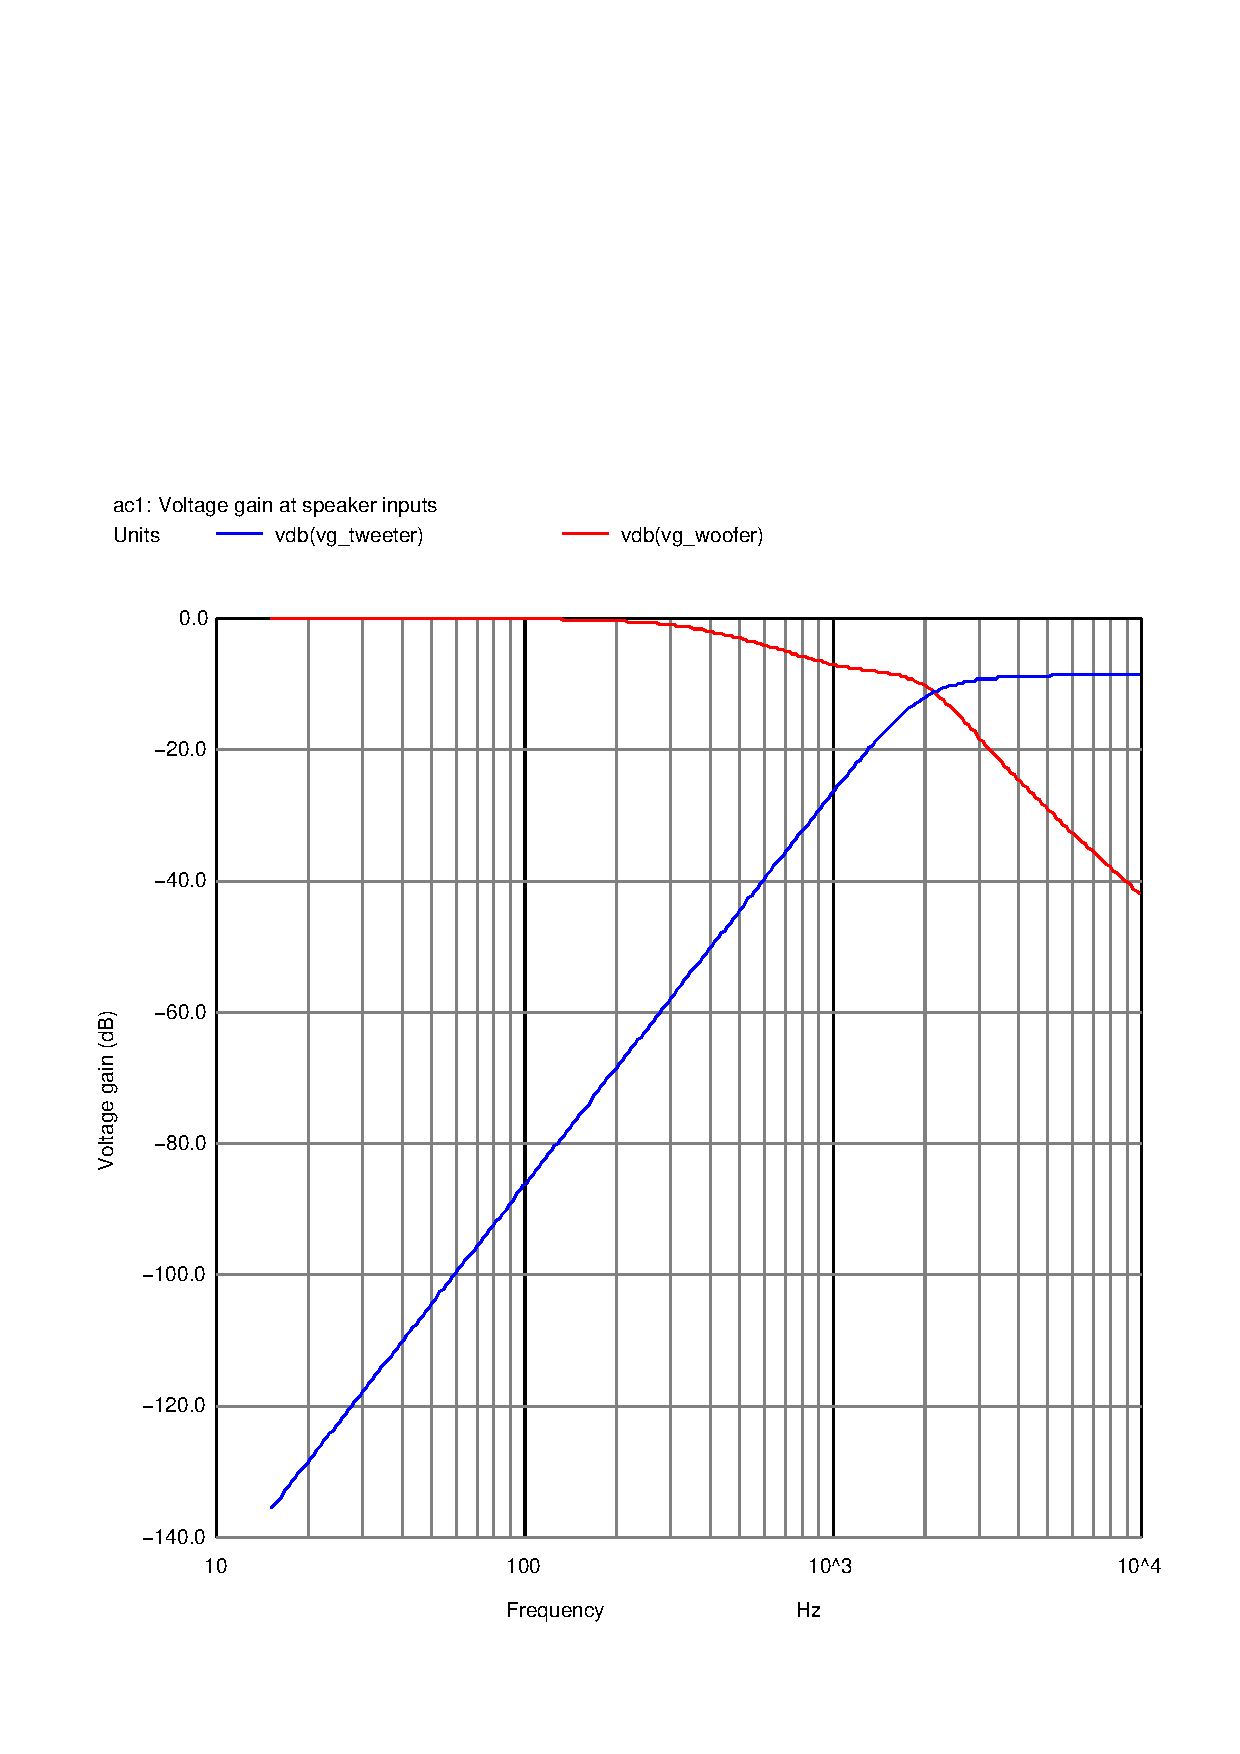
\includegraphics[scale=0.35,page=1]{../crossover/ngspice/gain.pdf}
	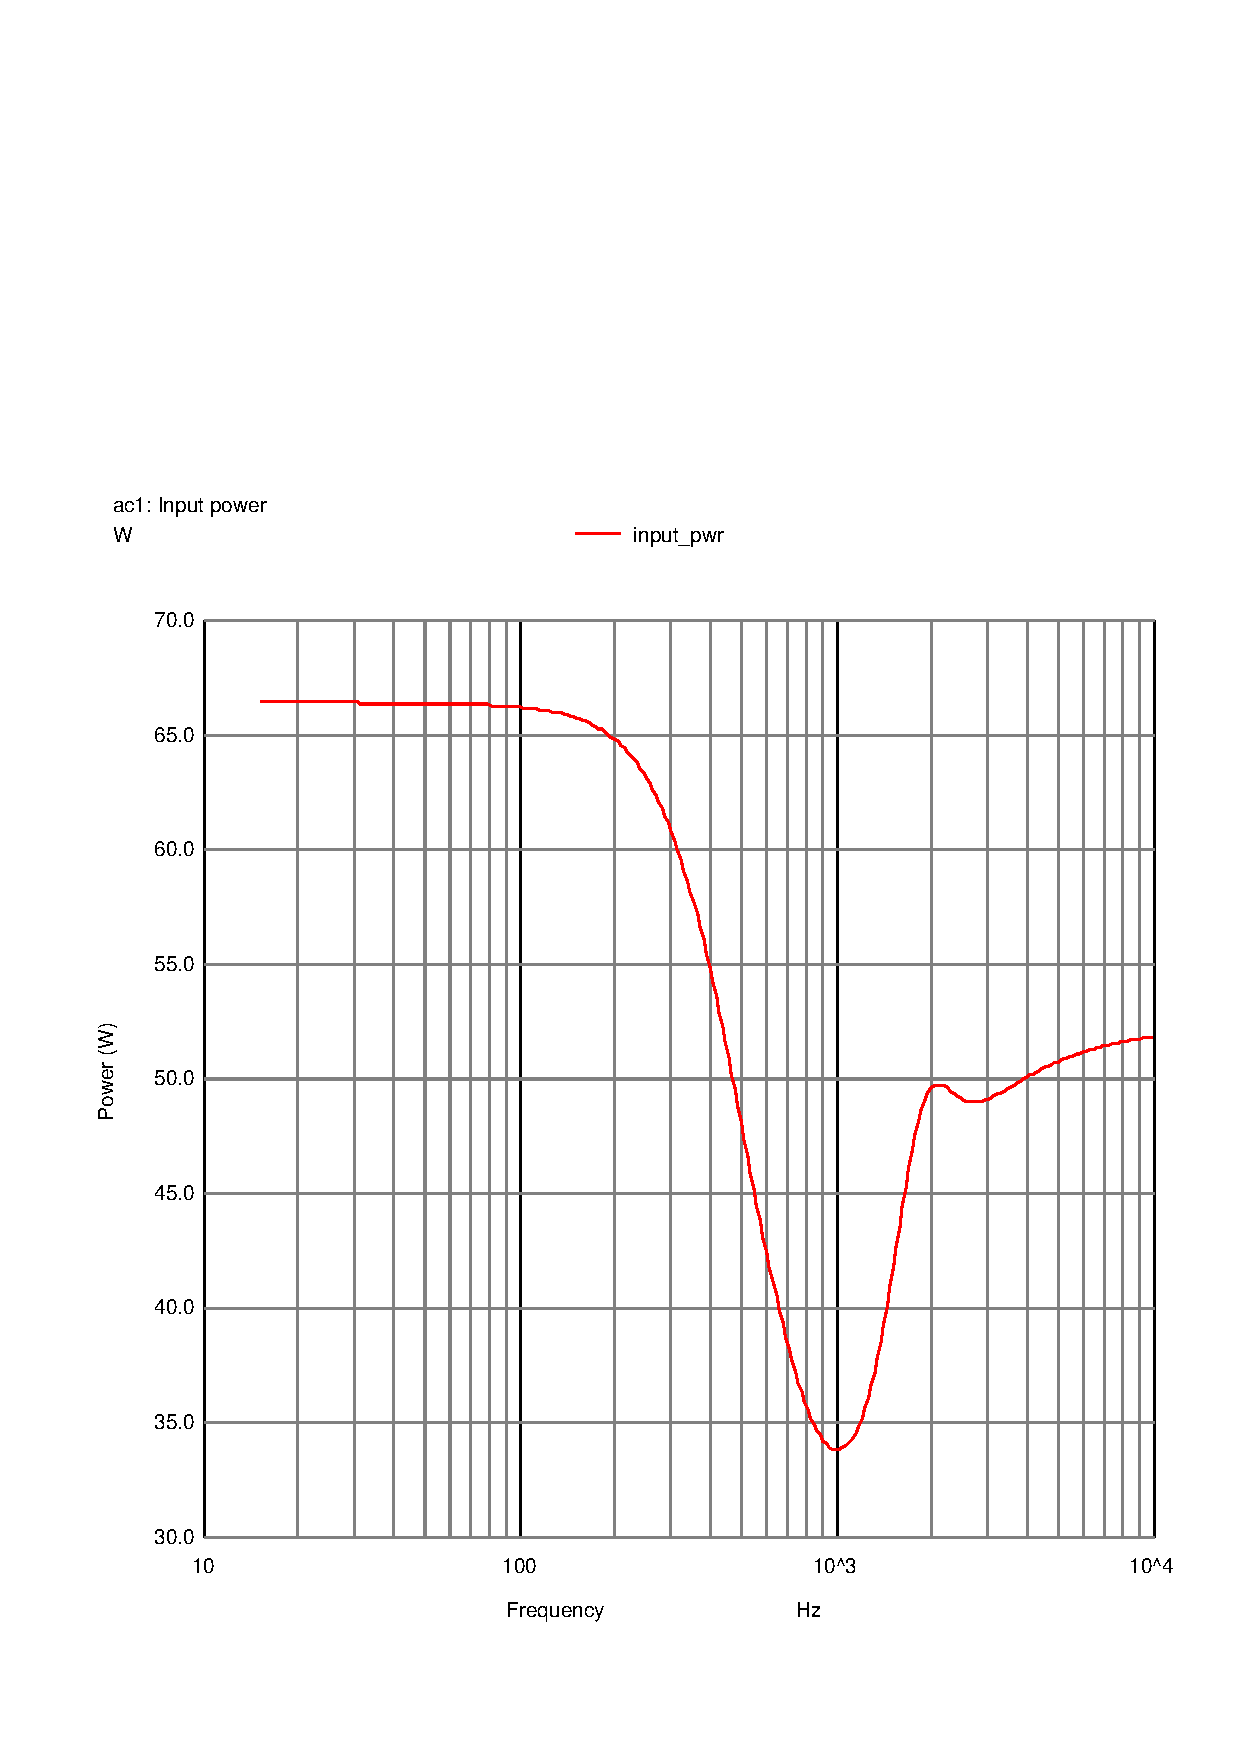
\includegraphics[scale=0.35,page=1]{../crossover/ngspice/in_pwr.pdf}
	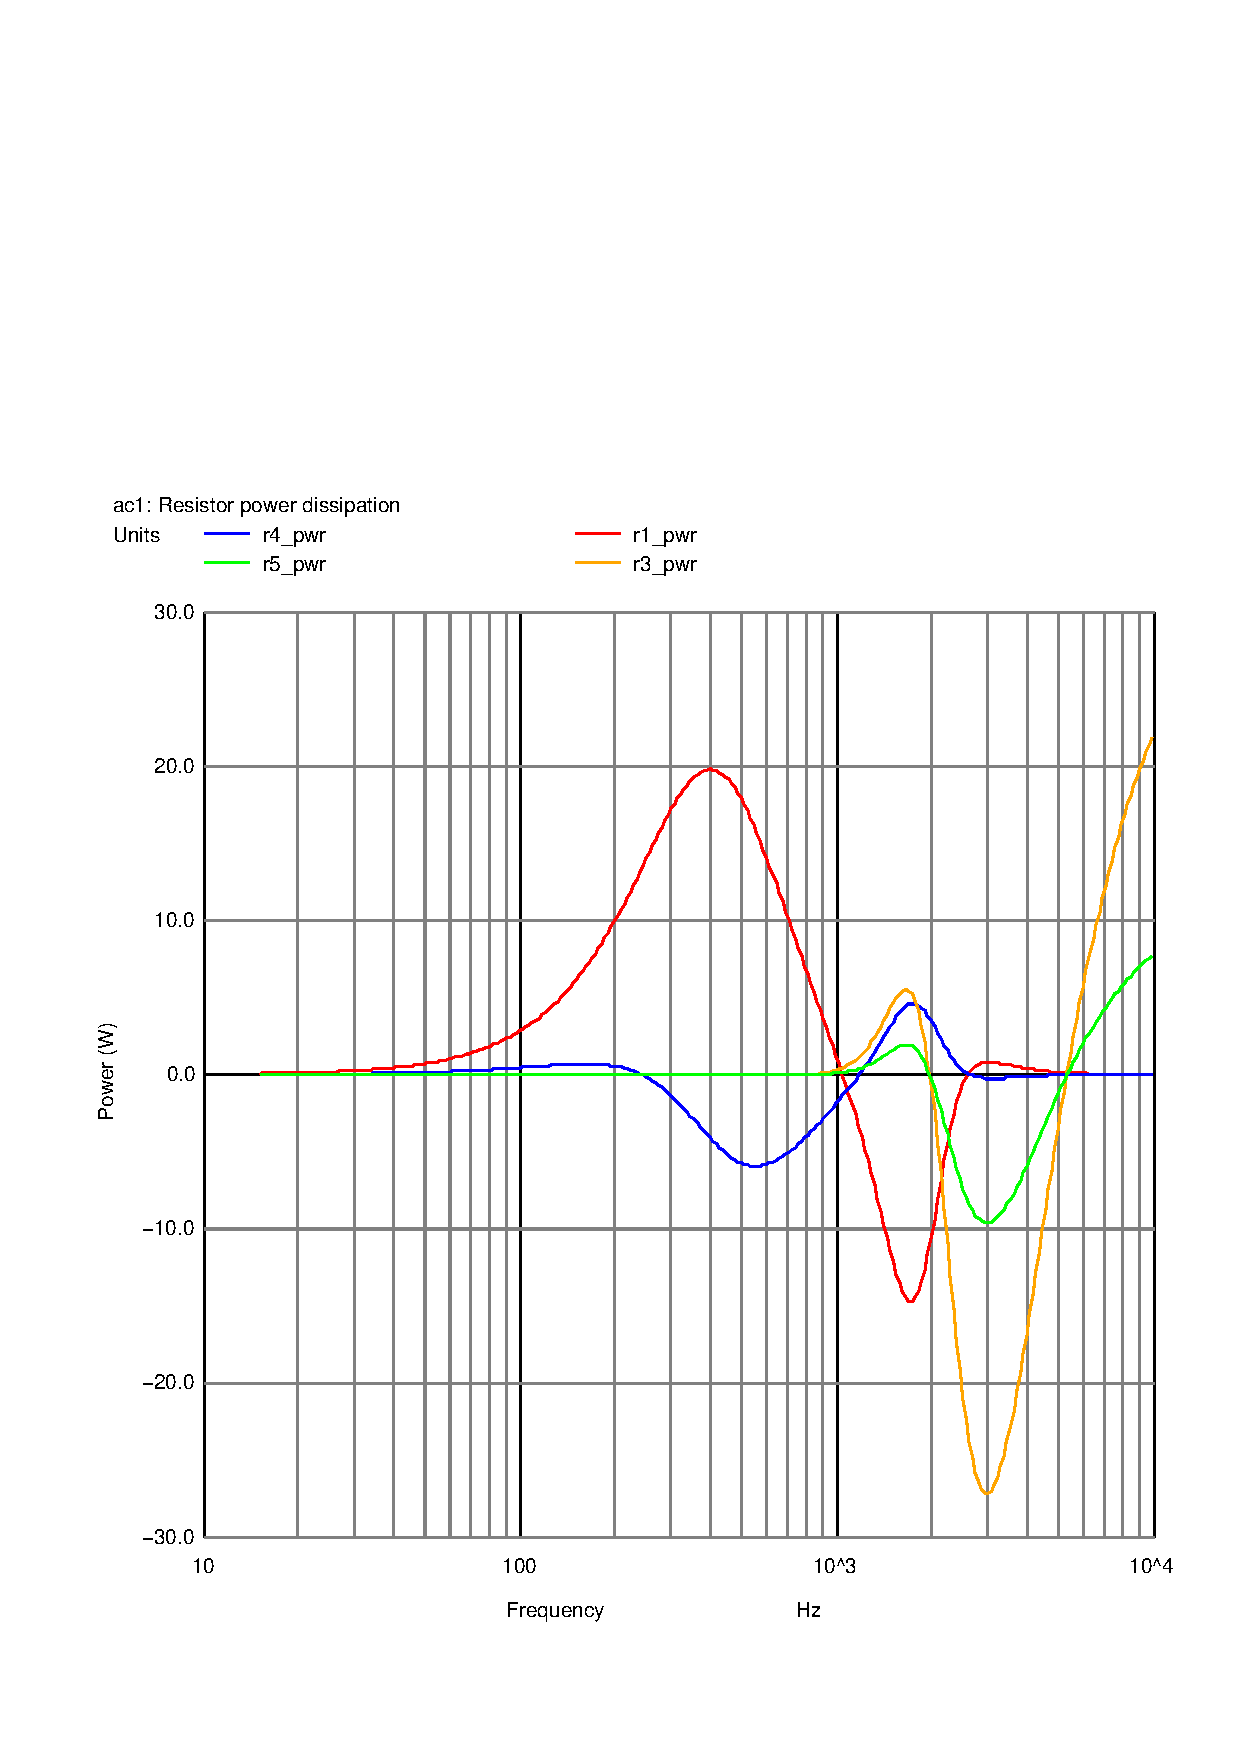
\includegraphics[scale=0.35,page=1]{../crossover/ngspice/r_pwr.pdf}
	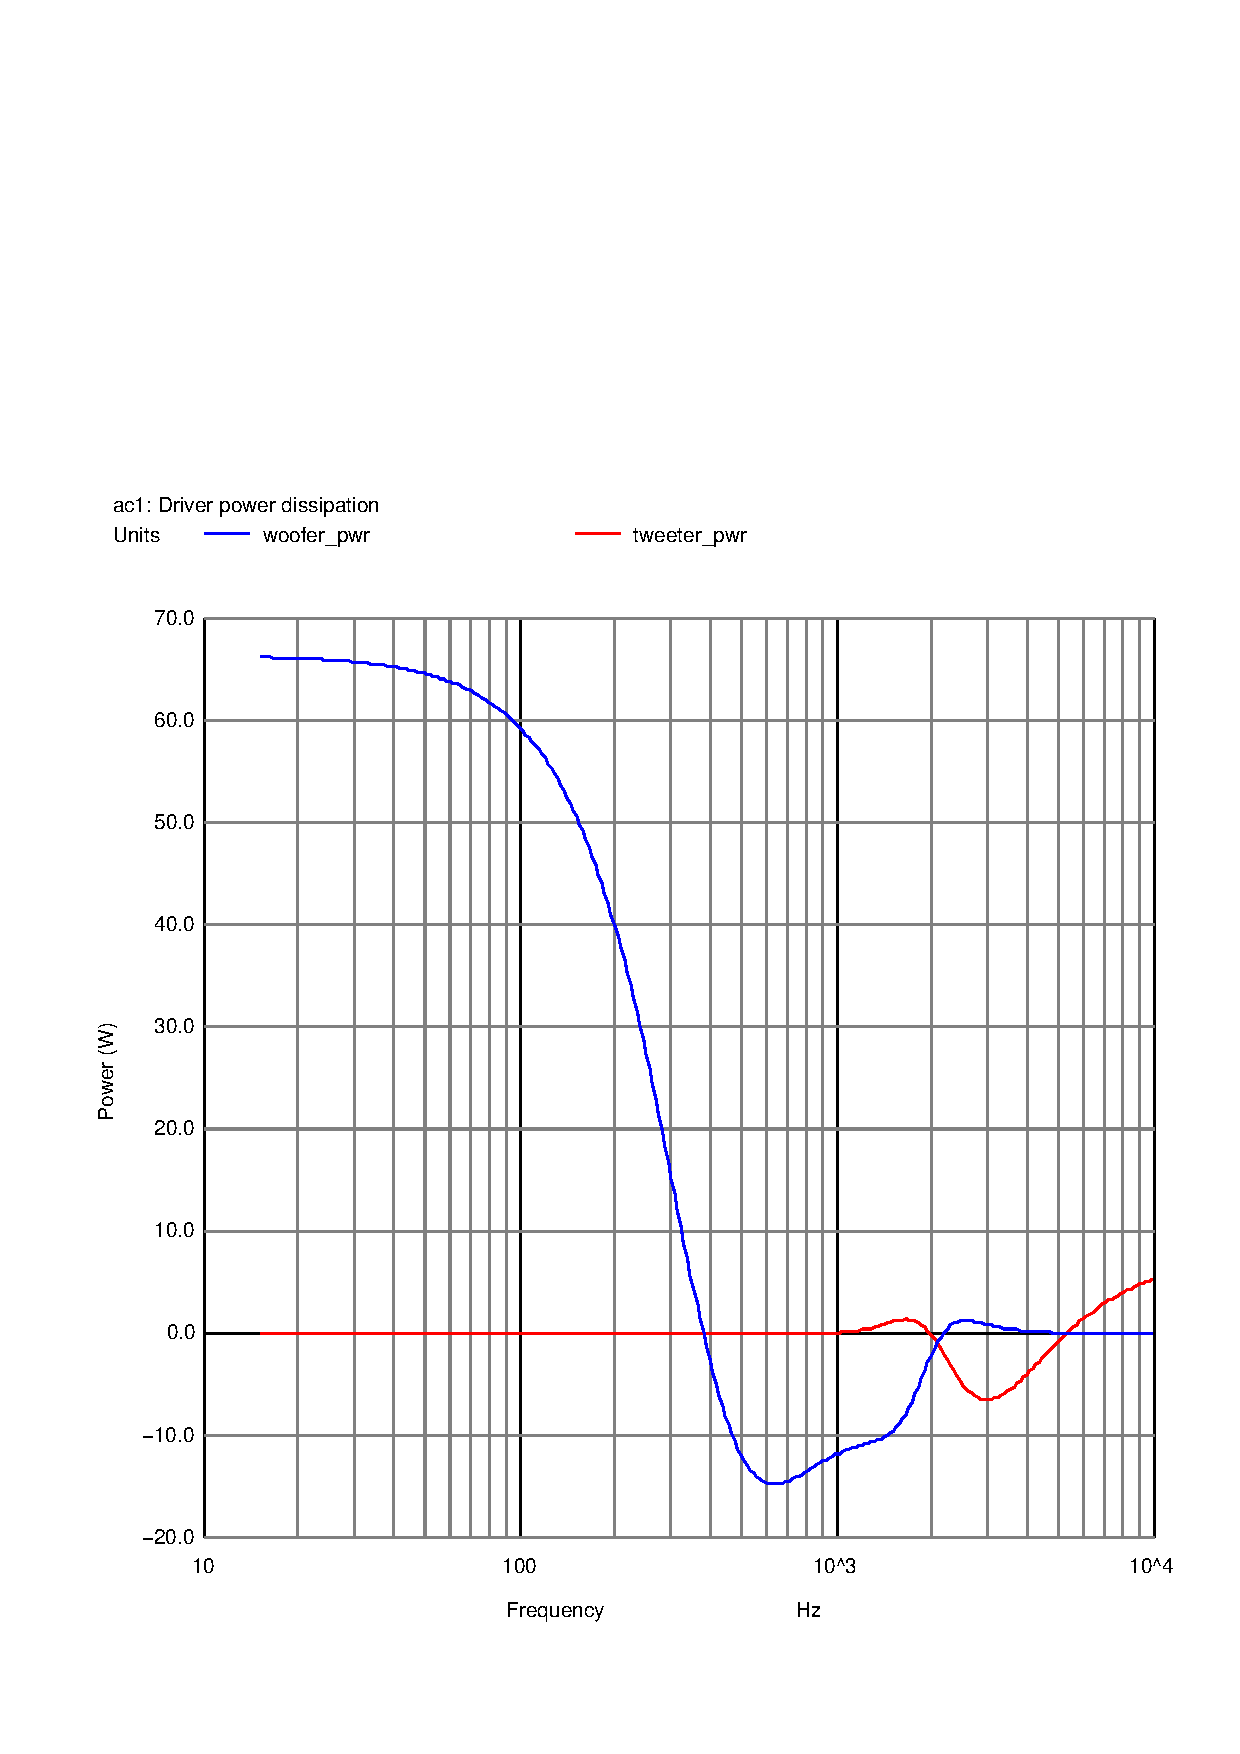
\includegraphics[scale=0.35,page=1]{../crossover/ngspice/spk_pwr.pdf}
	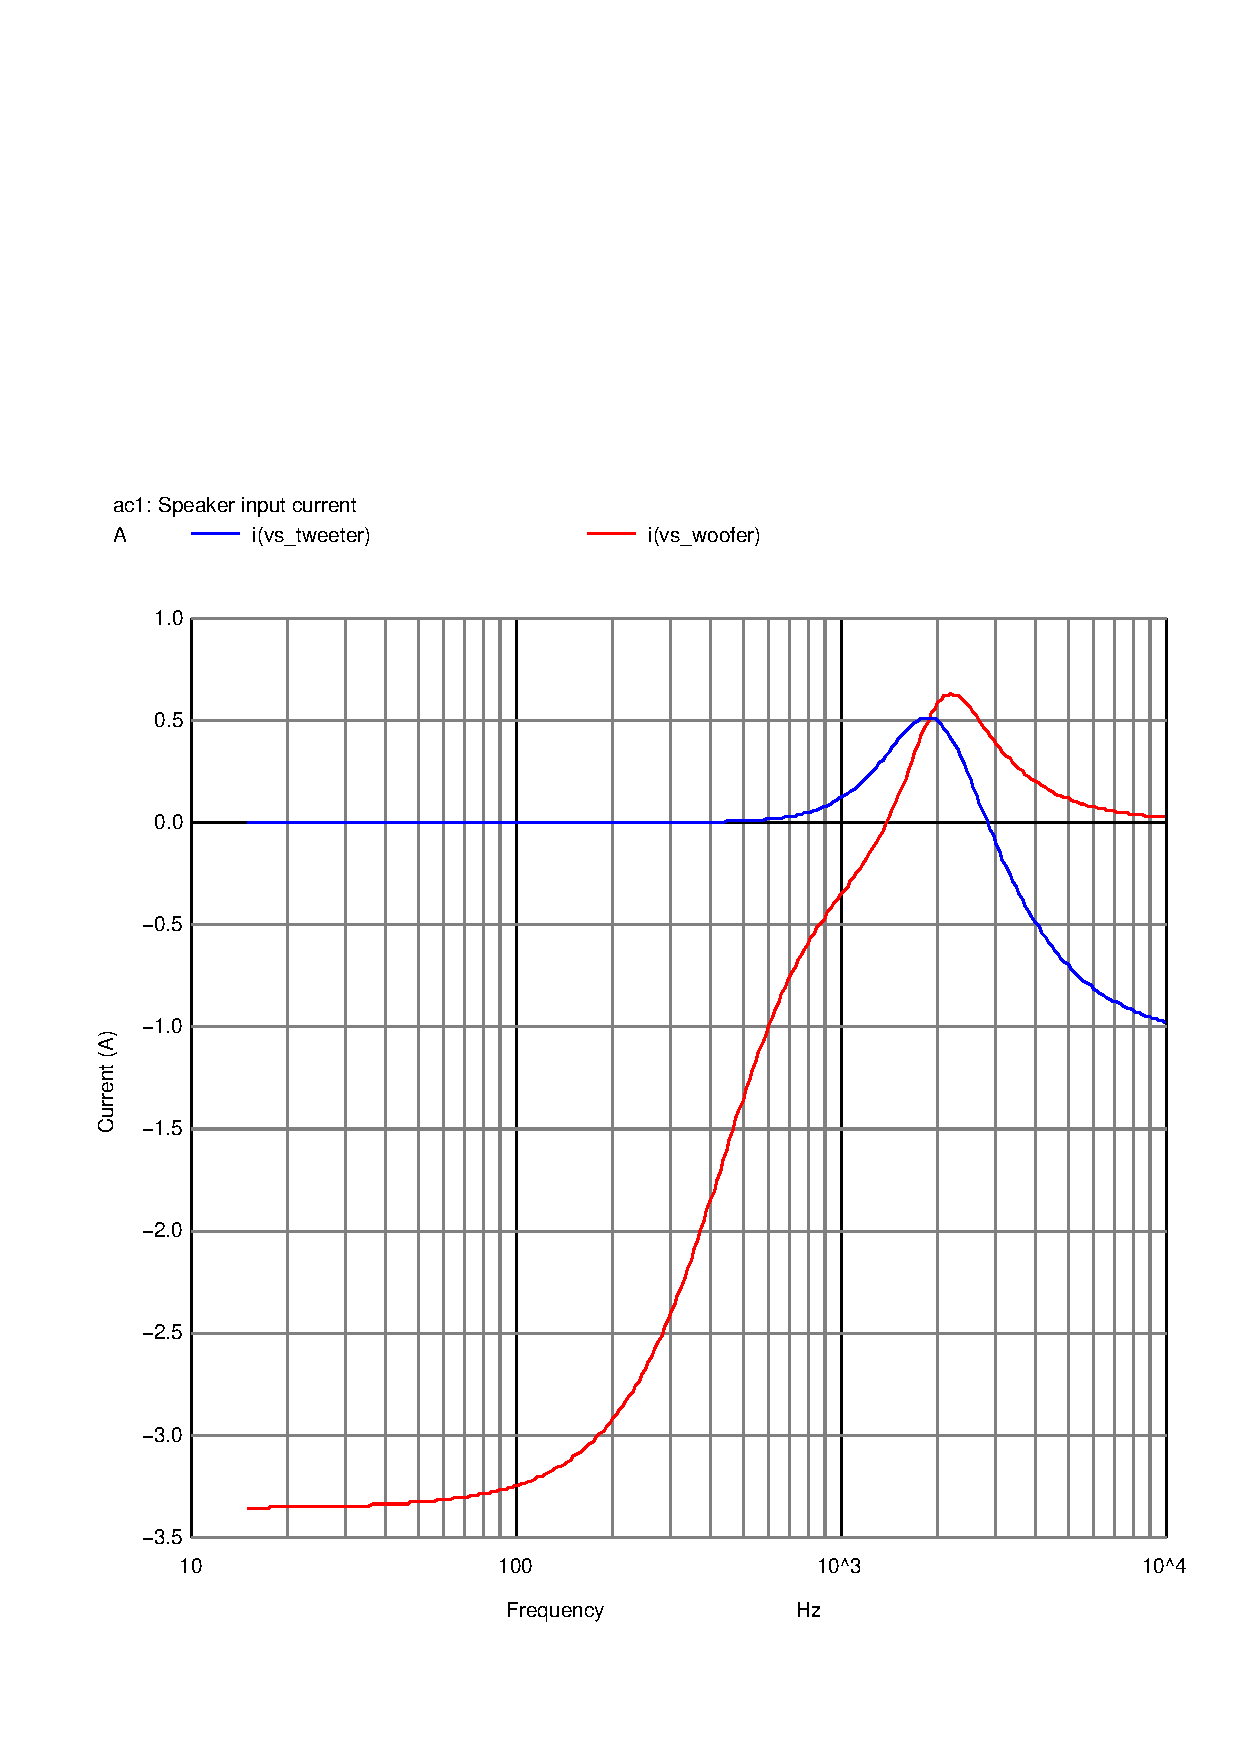
\includegraphics[scale=0.35,page=1]{../crossover/ngspice/in_current.pdf}
\end{multicols}

\end{document}
